\chapter{Hydrogel design for protein separation}\label{ch03}

In order to test the predictions of our bound-state diffusion model of selectivity, we needed to develop a biomaterial that could support bound diffusion and be used to test selectivity.  There are several biological examples which show selectivity that could be explained by bound-state diffusion, including nucleocytoplasmic transport, liquid-liquid phase separated droplets, diffusion of DNA-damage-repair proteins in the nucleus, and passage through mucus\cite{zhou12,witten17,hoiby10, rudolph18}.  We decided to focus on making a material that mimics the environment of the nuclear pore.

One of the attractions of the bound-state diffusion model is that it does not rely on the geometry of the selective material.  As long as the dimensions of the material are significantly larger than the protein diffusing through it, there is no practical difference between a nanoscale cylindrical pore and a macroscale bulk material.  For ease of fabrication and testing, we opted to design a bulk material for protein separation.

A hydrogel substrate was chosen as the basis of the nuclear pore mimic and protein fragments taken from FG Nups anchored into it.  Hydrogels are versatile materials, many of which are bio-compatible, many of whose properties can be easily tuned .  We used a hydrogel substrate to provide an inert scaffold to which fragments of FG Nups were conjugated.  These Nups were conjugated to the hydrogel at one end and free at the other, mimicking the arrangement found in the nuclear pore and providing a mechanism of tethered bound diffusion.  The properties of these Nups, such as their length, number of transport factor binding motifs, and propensity towards aggregation, can be easily varied in order to test how these properties impact bound-state diffusion and thus protein selectivity.

This hydrogel model is therefore the simplest way to make a material to explore the effects of bound diffusion on protein separation.  While it is inspired by the nuclear pore, the goal is not to directly reproduce the mechanism of nucleocytoplasmic transport.  Instead, we hoped to show that bound-state diffusion was measurable and controllable in a biomaterial, paving the way for molecular filters that might make use of this principle.

Over the course of making these materials, we ran into several significant roadblocks.  Although hydrogels with a wide range of properties have been well-studied, gels suitable for protein separation are harder to come by.  They require an intermediate pore size, large enough that the diffusion of a protein is not significantly hindered by the presence of the hydrogel meshwork, but small enough that the Nup peptides can easily reach the protein as it diffuses.  This average pore size of 5-20 nm is difficult to find, though much smaller and much larger pores are easy to make.  The problem of pore size is made more difficult by the need to create a well-sealed hydrogel barrier in order to separate proteins; such a barrier must necessarily be confined and therefore unable to swell to its equilibrium size. The creation of a hydrogel for selective protein separation poses many stringent requirements, often in competition with each other.  This chapter describes the setbacks we faced and the progress we have made towards creating a hydrogel-based biomaterial suitable for selective separation of proteins.


\section{Hydrogel fabrication}
\label{sec:hydrogel-fabrication}

\begin{figure}
\caption{Overview of hydrogel fabrication and fluorescent protein influx. A precursor solution is mixed, containing hydrogel monomers, crosslinkers, a photoinitiator, and the Nup fragment.  Upon exposure to UV light, the precursor solution crosslinks, and one end of each Nup is conjugated to the hydrogel.  The diffusion of a fluorescently-tagged transport factor can then be compared to that of a similarly-sized inert fluorescent protein.}
\centering
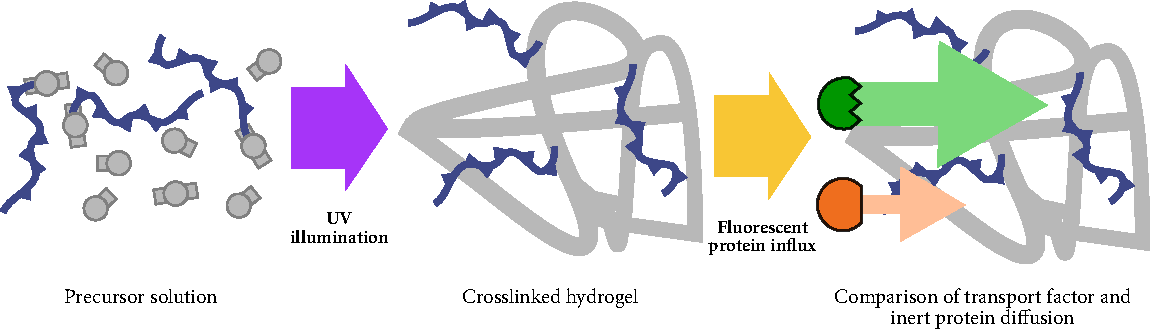
\includegraphics[width=\textwidth]{figs/ch03/precursor}
\label{fig:precursor}
\end{figure}

A wide range of hydrogels systems have been well-studied.  Many are not suitable for the addition of proteins, but both PEG and acrylamide hydrogels, among others, can be crosslinked in an aqueous solution that does not harm proteins.  We used both PEG and acrylamide hydrogels in our diffusion experiments.  Thanks to Stephanie Bryant, Sadhana Sharma, Christopher Bowman, Danielle Konetski, and Benjamin Fairbanks for their help as we learned to make these hydrogels.

Whether using PEG or acrylamide, the basic hydrogel fabrication procedure was the same (Fig.~\ref{fig:precursor}).  First, a precursor solution was mixed, which contained the hydrogel monomer, a crosslinker, a radical generator, and the Nup fragment, labeled with a reactive group at one end that would conjugate it to the hydrogel.  The radical generator was almost always a photoinitiator, which caused the precursor solution to crosslink when exposed to UV illumination.  In a few cases, a chemical initiator was used, in which case the precursor solution crosslinked 10-30 minutes after mixing.  By the end of the crosslinking process, the hydrogel contained Nup fragments tethered to the gel at one end, mimicking the arrangement of Nups in the nuclear pore and providing a mechanism of tethered bound diffusion for transport factors but not for non-binding inert proteins.  The diffusion of both types of protein within the hydrogel could then be quantified using fluorescence microscopy.

There were four major components to the precursor solution: monomers, crosslinkers, initiators, and Nup fragments.  To an extent, these components can be chosen independently of each other.  Bisacrylamide or PEG-diacrylate crosslinkers must be used with acrylamide monomers, and PEG-dithiol crosslinkers with PEG-norbornene monomers, but the initiators and Nup fragments can be varied.  There are many variations on crosslinker length as well, leading to a wide variety of possible hydrogels even using a relatively small set of components.

The PEG hydrogels made use of 20-kD 8-armed PEG-norbornene monomers (synthesized by the Bryant lab and Nathan Crossette) and either a 1-kD or 8-kD PEG-dithiol crosslinker (Sigma) (Fig.~\ref{fig:monomer-crosslinker}).  To conjugate the Nup fragment to the PEG hydrogels, a cysteine was engineered at one end (lookup: which end?).  Both the crosslinker and Nup fragment made use of Michael-thiol ``click'' chemistry \cite{chatani14}\cite{nair14}.

The acrylamide hydrogels used an acrylamide monomer and bisacrylamide crosslinker (BioRad) (Fig.~\ref{fig:monomer-crosslinker}).  An additional step was needed to prepare the Nup fragment for tethering to the hydrogel: either bisacrylamide or 700-Da PEG-diacrylate (lookup: Sigma) was conjugated to the terminal cysteine (see Appendix~\ref{appx:bis-labeling}).

\begin{SCfigure}
\caption{Chemical structures of monomers and crosslinkers for PEG and acrylamide hydrogels. The total molecular weight of the 8-armed PEG-norbornene was 20 kD, and either a 1-kD or 8-kD PEG dithiol crosslinker was used.  Structures from Sigma and CreativePEGWorks.}
\centering
\includegraphics[width=0.7\textwidth]{figs/ch03/monomer-and-crosslinker}
\label{fig:monomer-crosslinker}
\end{SCfigure}

Regardless of the monomers and crosslinkers used, a radical generator is needed to initiate polymerization.  We used either a photoinitiator, activated by UV light, or a chemical initiator system which began polymerization upon its addition to the precursor solution.  Both systems have advantages: Photoinitiators are useful for patterned polymerization using photomasks and allow the precursor to be mixed prior to polymerization, while chemical crosslinkers do not require careful protection from light.  We nearly always used a photoinitiator.

Two photoinitiators were tested: 1-[4-(2-hydroxyethoxy)-phenyl]-2-hydroxy-2-methyl-1-propane-1-one (commercially known as Irgacure 2959) and lithium phenyl-2,4,6-trimethylbenzoylphosphinate (LAP). %http://www.xtgchem.cn/upload/20110629045632.PDF
Figure~\ref{fig:initiators} (A) and (B) shows the absorption spectra of each photoinitiator and that of its cleavage products \cite{fairbanks09}.  LAP has an absorbance peak in the near-IR / violet range, is highly water-soluble, and is more effective at crosslinking, so it was used most of the time.  However, due to its absorbance into the visible range, care must be taken to protect solutions containing LAP from ambient light wherever possible.  Our LAP was synthesized by the Bryant lab, but it is now commercially available from Sigma as well.

\begin{figure}
\caption{Absorption spectra of (A) Irgacure 2959 and (B) LAP (solid lines) and with that of their cleavage products (dotted lines) \cite{fairbanks09}. (C) Chemical structures of the APS/TEMED crosslinking system. Structures from Sigma.}
\centering
\includegraphics[width=\textwidth]{figs/ch03/initiators}
\label{fig:initiators}
\end{figure}

An APS/TEMED chemical crosslinking system was occasionally used in place of the photoinitiator.  Large numbers of hydrogels can be polymerized at once in this way, without the need for a large area of uniform UV illumination.  Figure~\ref{fig:initiators} (C) gives the chemical structure of ammonium persulfate (APS) and N,N,N′,N′-tetramethylethylenediamine (TEMED).  APS is the radical generator, and TEMED accelerates the radical formation.  The time to polymerize can be controlled by adjusting the concentration of both components (lookup: put this info in an appendix?).

It should be noted that the presence of oxygen inhibits all the initiators discussed above.  Precursor solutions were degassed for 10 minutes before use in a vaccum desiccator and polymerized no more than 10 minutes after degassing.

When a photoinitator was used, the hydrogels were polymerized using UV illumination at either (lookup: LED wavelength) (lookup: Thorlabs LED model) or 405 nm (laser on A1R confocal microscope) inside flow chambers as described in Sec.~\ref{sec:flow-chambers}.  The typical intensity of the LED was (lookup) and the typical crosslinking time 30 s.  Depending on the situation, photomasks were used to selectively expose regions of precursor to UV, or entire droplets of precursor solution were polymerized in an otherwise-empty chamber (Fig.~\ref{fig:photomask}).  After crosslinking, hydrogels were rinsed with 10-100 times their volume with buffer and allowed to soak in fresh buffer solution overnight at 4$^\circ$C in order to approach swelling equilibrium and remove any remaining precursor solution.

\begin{figure}
\caption{Procedure for photopolymerization with (A) or without (B) a photomask. (A) A flow chamber is filled with precursor solution.  The photomask is placed to hide all areas that should not be crosslinked, and the chamber is exposed to UV illumination.  Excess precursor solution is removed with a buffer rinse. (B) Microliter droplets of precursor solution are pipetted onto the slide surface before the chamber is assembled.  After assembly, the chamber is exposed to UV illumination.  The chamber is then filled with buffer.}
\centering
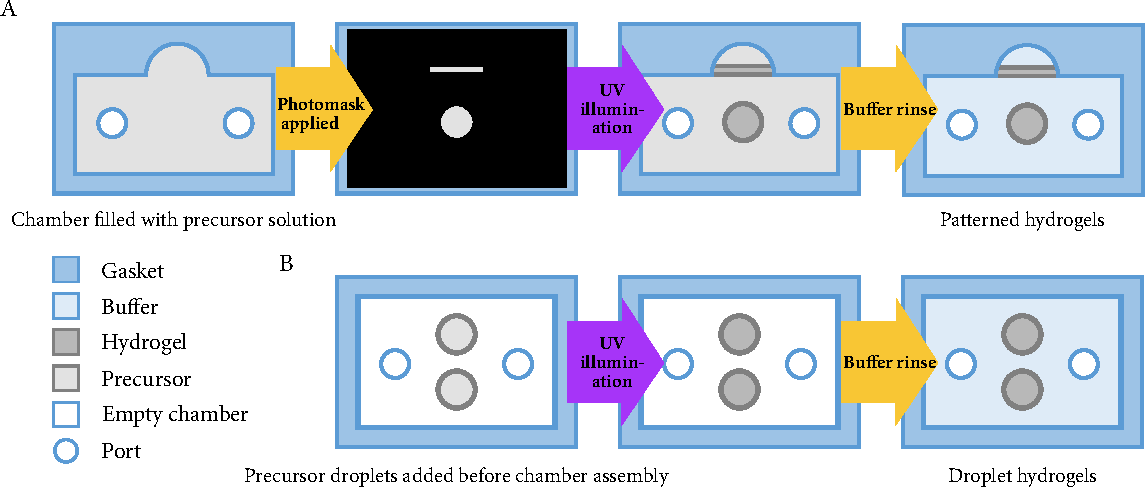
\includegraphics[width=\textwidth]{figs/ch03/photomask}
\label{fig:photomask}
\end{figure}

Following the buffer soak, typically a fluorescent solution of proteins was added to the gels.  Usually this consisted of a transport factor (typically NTF2) and a similarly-sized inert protein (typically the red fluorescent protein mCherry).  A typical experiment consisted of a video at 4x or 10x magnification of the hydrogel, reservoir chamber, and (if applicable) an outlet/inner reservoir which slowly accumulated protein as it passed through the gel.  Experiments ranged from 1-24 hours, with 2 hours being the most common.  Typical data produced was a plot of accumulation in the inner reservoir or hydrogel over the course of the experiment, as well as a concentration profile through the gel and inner reservoir.  Experiments are described in greater detail in Chapter~\ref{ch:bound-diffusion}.

% Appendix - detailed gel-making procedureThe acrylamide hydrogels were made in an aqueous buffer with dilutions of a 30\% solution of acrylamide and bis-acrylamide (29:1) ratio, the Nup fragment, and either a chemical initiator system (ammonium persulfate (APS) and N,N,N',N'-Tetramethylethylenediamine (TEMED)) or LAP. 

%\subsection{Preparing Nup fragment for conjugation to acrylamide gels} -appendix

% appendix - effect of varying APS and TEMED concentration

% appendix - sample precursor solution recipes

% appendix - FSFG growth, purification, lyophilization
%\label{sec:bisRxn}

\section{Flow chamber fabrication}
\label{sec:flow-chambers}

The hydrogels were usually crosslinked in microfluidic flow chambers as shown in Fig.~\ref{fig:chamber-geometries} (A).  The thin chambers ensured that the top and bottom of the gel were sealed, so that transport factors and inert proteins could enter the gel only by diffusing into it.  The small chamber size also reduced the quantity of transport factor and inert protein solution needed.  Finally, the chambers were designed to be easily mounted on a microscope stage for recording experiments.

\begin{figure}
\caption{Flow chamber design and geometries.  (A) Schematic of the most common flow chamber, showing slide, coverslip, gasket, ports, and hydrogels.  (B)-(F) Common hydrogel geometries.  Those in the left-hand column are suitable for selectivity measurements as well as diffusion measurements, while the right-hand column cannot be used to measure selectivity.}
\centering
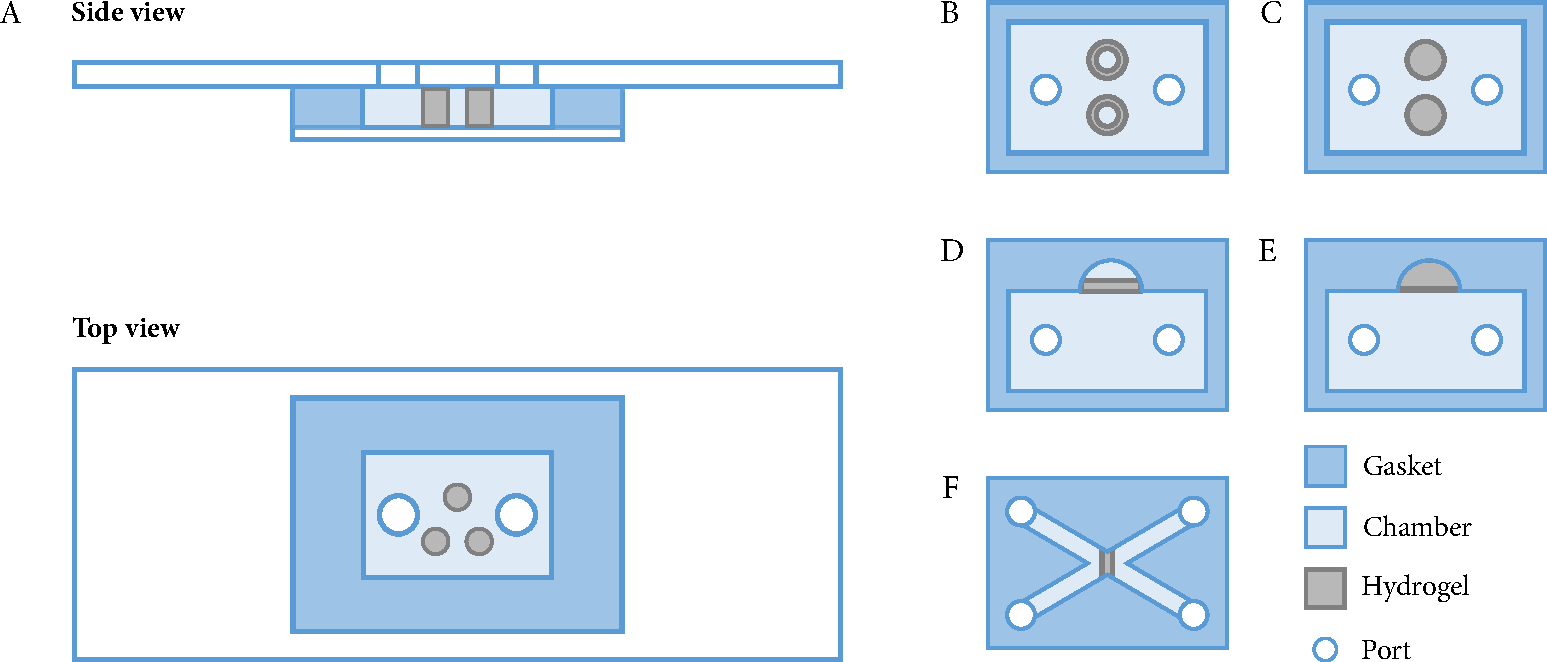
\includegraphics[width=\textwidth]{figs/ch03/methods-cartoon}
\label{fig:chamber-geometries}
\end{figure}

The basic flow chamber design consisted of an acrylic slide, patterned spacer or gasket, and coverslip, stacked and sealed together.  Ports were almost always drilled in the plastic slide before chamber assembly, in order to allow the chamber to be filled and emptied.  Several methods of fabricating the gaskets and ports were tested in order to optimize the watertightness and longevity of the chambers as well as the ease of fabrication and re-use.

In particular, several materials were attempted for the gasket that determined the height and shape of the chamber.  The simplest was double-stick tape, which could be used as a single width or cut into shape with a razor.  The double-stick tape chambers were thin (70 $\mu$m per tape layer), of reliable thickness, and quick to make.  However, they often leaked or dried over the course of several hours.  Since many experiments take several days from preparation to finish, double-stick tape chambers were not usually not sufficient.

Norland Optical Adhesive (NOA), a liquid adhesive which cures upon exposure to UV, was used in another style of flow chamber.  Thin semi-cured NOA layers can be molded and used as ``stickers'' to build flow chambers \cite{bartolo08, paustian13}.  This procedure is outlined in Fig.~\ref{fig:stickers} and relies on the inhibition of curing by oxygen.  A droplet of NOA is sandwiched between a glass coverslip and a PDMS mold, which is permeable to oxygen. The NOA is briefly (approximately 3 seconds at lookup: intensity) cured, though a thin layer remains uncured due to the presence of oxygen at the adhesive's surface. The PDMS mold is carefully peeled away, and the coverslip with NOA sticker is attached to the slide and sealed.  The NOA is then fully cured and the chamber rinsed with ethanol to remove any uncured NOA remaining. Rather than applying NOA directly to the mold, as shown in Fig.~\ref{fig:stickers} (A), it is also possible to seal the mold to the coverslip and wick NOA into the hollows (Fig.~\ref{fig:stickers} (B).  This method is more error-prone and time-consuming but results in a flow chamber with glass on the top surface instead of NOA.  Proteins are often less inclined to stick to the glass surface than to NOA.

\begin{figure}
\caption{Microfluidic sticker fabrication from \cite{bartolo08}. (A) A PDMS mold is used to shape an NOA droplet on a flat slide.  The NOA is briefly cured but retains a sticky surface.  (B) NOA can also be wicked into a PDMS mold. (C) The NOA sticker is placed onto a permanent surface, sealed, and cured entirely.}
\centering
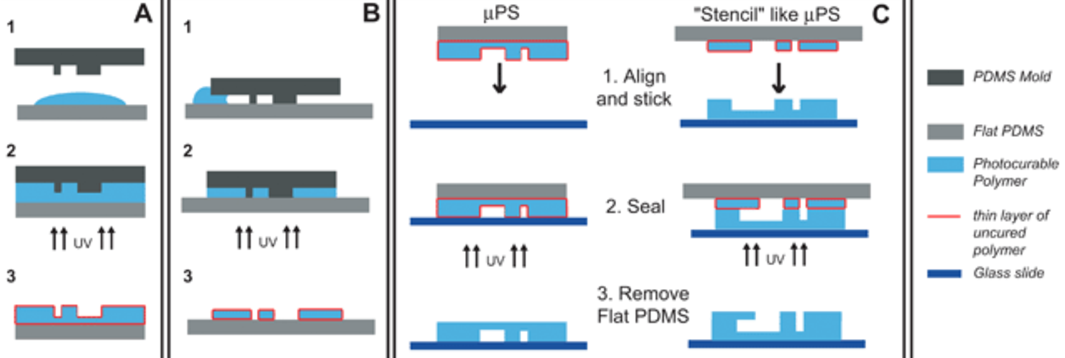
\includegraphics[width=0.8\textwidth]{figs/ch03/sticker-bartolo.pdf}
\label{fig:stickers}
\end{figure}

PDMS molds for the NOA stickers were made cheaply with (lookup) 0.5-mm resolution using a Silhouette craft cutter (lookup brand exactly).  After creating a template with the craft cutter's software, the design was cut into a layer of packing tape that had been carefully applied to a large glass slide. The unwanted tape was peeled away using a razor and tweezers, leaving a depression where the chamber would eventually sit, and the slide used as the reverse-mold for a PDMS mold.

NOA-chambers are much more resistant to drying than double-stick-tape chambers, and can withstand the largest pressure and most rapid flow.  On the other hand, they are significantly more difficult to make and cannot be re-used.  For most experiments, where rapid flow is not necessary, PDMS gaskets were the most useful.  Chambers made with PDMS gaskets are thicker (100-400 $\mu$m) than the other varieties and their thickness is not as reproducible, but they are easy to reuse, often can last several days without drying out, and are quick to assemble.  

PDMS gaskets were made by preparing the volume of PDMS mixture needed to create a layer of a given thickness in a standard Petri dish.  Once the PDMS had been thoroughly mixed, degassed, and spread evenly across the dish, it was cured for an hour at 70$^\circ$ and cut into shape with a razor.  Measurement with a micrometer indicated that the nominally 400-$\mu$m-thick PDMS film had an error of no more than 10\%.  This thickness proved to be optimal for sealing to both the acrylic slide and glass coverslip, as well as easily re-usable after thorough cleaning with ethanol.

While plasma-bonding the PDMS to the glass was tested, it proved unreliable.  As long as the chamber was not subjected to high pressures, an adequate seal formed without additional treatment if all materials were cleaned with ethanol and dried with house air before use. Likewise, silanation of the glass was attempted, in order to bond the hydrogel more securely to the top and bottom chamber surfaces, but it was not needed.  The gels sealed well to the chamber as long as they were in contact with the surfaces while crosslinking.  However, crosslinking the hydrogels on PDMS and then transferring them to the chamber resulted in a poor seal.  In consequence, almost all experiments were run using gels that had been crosslinked inside a chamber.

The ports were another point of concern for the watertightness of the chambers.  If liquid needed to be flowed through a chamber at an appreciable speed, short lengths of PEEK tubing were superglued into the ports and fitted with Tygon tubing, which was then attached to a blunt-tipped syringe.  For sufficiently gentle flows, however, ports were left simply as holes in the plastic slide and the chamber filled by pipette.  After the chamber was filled, PEEK tubing ports were sealed with parafilm, and holes were sealed with a flat slab of clean PDMS.

Finally, portless thin chambers were used ocasionally, such as for attempting fluorescence recovery after photobleaching (FRAP) using a confocal microscope.  To make these chambers, microliter or smaller droplets of precursor solution containing 6-$\mu$m glass spacer beads were placed on glass slides and covered with a coverslip.  The hydrogel was crosslinked and fluorescent protein solution wicked into the chamber.  The chamber was sealed with valap (a 1:1:1 ratio of vaseline, lanolin, and paraffin which easily melts over a burner and re-solidifies rapidly).  Such chambers last several hours on the microscope without drying but should not be used for longer experiments.

\section{Hydrogel geometries}

Our ultimate goal was testing protein separation by monitoring their passage into and through a selective material.  In order to truly measure selectivity, the accumulation of proteins in an outlet reservoir beyond the test material must be measured, not just influx into the material.  Many hydrogel and flow chamber geometries were tested in search of a setup that would allow selectivity, as well as free and bound diffusion, to be directly observed.

The limiting factors were the resolution of patterned hydrogel features, the size and accessibility of the outlets, and the equilibrium swelling of the hydrogels.  Attempts to improve one of these factors typically led to worse outcomes for the others.  Two major classes of hydrogel geometry emerged: those with an outlet reservoir, and those without.  The hydrogels without an outlet reservoir cannot be used to directly measure the gels' selectivity, but diffusion constants for the inert protein and transport factors can still be determined.  Chapter~\ref{ch:bound-diffusion} details the results of bound-state-diffusion experiments using no-outlet hydrogels.

The hydrogel geometries that contained an outlet reservoir are shown in Fig.~\ref{fig:chamber-geometries} (B), (D), and (F).  Ring-shaped gels (B) provide a small outlet reservoir, which is quick to equilibrate.  They were fabricated using a confocal microscope (Sec.~\ref{sec:confocal-crosslinking}) or using PDMS molds 1-5 mm in diameter.  While these rings would have been ideal for selectivity measurements, we were never able to work out a procedure that would result in artifact-free, well-sealed rings.

Fig.~\ref{fig:chamber-geometries} (D) features a portless outlet reservoir which is much smaller than the inlet.  As with the ring gels, these outlets are quick to equilibrate and their precise volume can be calculated, as the entire outlet is in the field of view of a 4x objective.  A thin hydrogel bar was polymerized using a photomask, separating the inlet and outlet reservoirs.  Without ports in the outlet, the chamber was soaked in buffer for 24 hours to remove the remaining precursor solution from the outlet.  The inlet could then be filled with a fluorescent protein solution and accumulation in the outlet measured over time.  Unfortunately, it's likely that the outlet itself was lightly crosslinked, no matter how carefully we used the photomask.  See Sec.~\ref{sec:confocal-crosslinking} for more evidence of stray crosslinking.  Additionally, the hydrogel bars were of irreproducible thickness (50-200 $\mu$m) and swelled or buckled unpredictably.  Ultimately, the lack of reproducibility between replicates made this geometry unusable.

Finally, Fig.~\ref{fig:chamber-geometries} (F) shows an x-shaped chamber with four ports.  A thin bar of hydrogel was polymerized at the junction of the arms using a photomask.  The inlet and outlet reservoirs are approximately the same size, leading to slow equilibration in the outlet.  The precise volume of the outlet is impossible to determine, as the arms are usually partly filled.  Additionally, these chambers must be made using NOA stickers, which are difficult to use, and they tend to dry rapidly.  The x-chamber geometry is therefore not useful except in specialized situations.  A slightly more helpful version is the counter-propagating flow chamber shown in Fig.~\ref{fig:chamber-geometries} (G).  In this version, the hydrogel bar is as long as possible, creating a ``hydrogel window'' that separates the two arms of the chamber.  While this setup was never used to test protein selectivity, in principle a counter-propagating flow can be established using syringe pumps in order to simulate constant concentration in infinite inlet and outlet reservoirs while using a limited amount of material. A similar setup is demonstrated in \cite{paustian13}.

The no-outlet hydrogel geometries shown in Fig~\ref{fig:chamber-geometries} (C) and (E) are much simpler to make but do not allow for measurement of protein selectivity.  Panel (E) shows a variation on the small-outlet chamber in which the outlet is filled with hydrogel and crosslinked using a photomask. Finally, the droplet gels in panel (C) were added to the chamber before assembly and crosslinked without a mask (Fig.~\ref{fig:photomask} (B)).  These are the only hydrogels which were made without a mask, which greatly reduced the irreproducible edge effects (also seen in Sec.~\ref{sec:confocal-crosslinking}).  Droplet gels have volumes of 0.5-2 $\mu$L and equilibrate 30-kDa proteins in 24-48 hours.  While these gels cannot be used to monitor selective transport through and exit from the gel, we can use them to measure the diffusion constants of proteins within the gel and the selective influx of transport factors.  Chapter~\ref{ch:bound-diffusion} focuses entirely on droplet hydrogels made in 400-$\mu$m-thick PDMS gasket chambers with two PEEK-less ports.

\section{FG Nup peptides}

The remaining components of the nuclear pore mimics are the FG Nup fragments which are tethered to the hydrogel scaffold.  There are a wide range of FG Nups, many of which can be deleted without apparently impacting nuclear transport \cite{strawn04, zeitler04}.  We chose to use Nsp1, an essential FG Nup for selective transport, as the basis for our Nup peptides. Like all FG Nups, Nsp1 has an ordered domain which anchors it to the channel wall, and a disordered region containing many FG motifs.  As a whole, the disordered region aggregates when isolated in buffer \cite{frey06, frey 07}.

\begin{SCfigure}
\caption{Nup fragments used in nuclear pore mimic experiments.  (A) The nuclear pore with FG Nups filling the central channel. (B) The essential FG Nup Nsp1 shown as a schematic sequence, with FG124 and FSFG fragments noted. (C) Variants of FSFG: FSFG-concat 1-cys with 6 FSFG motifs and a C-terminal cysteine; FSFG-concat 2-cys, as above but twice as long; SSSG-cys, like FSFG-concat 1-cys with the F's mutated to nonbinding S's.}
\centering
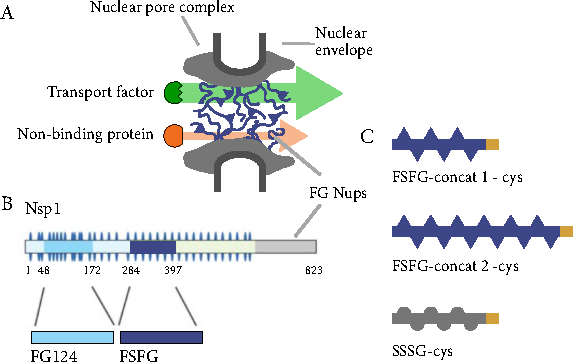
\includegraphics[width=0.6\textwidth]{figs/ch03/Nup-constructs.pdf}
\label{fig:Nups}
\end{SCfigure}

As shown in Fig.~\ref{fig:Nups}, we make use of two distinct fragments of Nsp1, denoted FSFG and FG124 \cite{hough15}.  Each are entirely disordered, are approximately 120 amino acids (14 kDa) in length, and contain multiple FG motifs.  FSFG is so called because it possesses six FSFG repeats.  It is extremely stable and unlikely to aggregate, remaining unaggregated throughout a wide range of buffers, pH values, concentrations, and crowding conditions.  As an additional advantage, FSFG can easily be expressed and purified.  The other Nup fragment, FG124, contains a variety of FG motifs (lookup).  If not kept in 7M guanidine hydrochloride, FG124 will aggregate over the course of several hours.  However, FG124 does not aggregate in the cellular environment, suggesting that Nsp1 itself may not be aggregated in the nuclear pore \cite{hough15}. 

Both FSFG and FG124 are expressed in Bl21 DE3 Gold cells in the pRSF plasmid, which is Kan resistant.  Each has a C-terminus 6xhis tag and are purified using a metal affinity column as described in Appendix~\ref{appx:protein-purification}.  They are unharmed by lyophilization and resuspension.

We have access to a wide library of FSFG and FG124 variants, few of which I helped to create. Many originate in Loren's old lab (lookup), and others were created by Andrea Egan, Nick Bax, Eric Verbeke, and myself. Table~\ref{table:Nups} shows the sequence of the most commonly-used Nup variants.

\begin{table}[b!]
\centering
  \caption{Library of FG Nup fragments.}
    \label{table:Nups}
    \begin{tabular}{p{3.5cm}p{4cm}p{8cm}}
      Description & Notes &Sequence \\
      \hline
      FSFG & (`FSFG concat-1') & MDNKTTNTTPSFSFGAKSDENKAGA TSKPAFSFGAKPEEKKDDNSSKPAFSF GAKSNEDKQDGTAKPAFSFGAKPAEKN NNETSKPAFSFGAKSDEKKDGDASKPAF SFGAKPDENKASATSKPALEHHHHHH\\
	FSFG cys & & \\
	FSFG 2-cys & Aggregates unless kept in reducing agent. & \\
	ybbR FSFG cys & Most often used for hydrogel experiments; ybbR tag is intended for site-specific labeling but not used in the hydrogel experiments.& \\
	FSFG concat-2 cys & & \\
	FSFG concat-3 cys & Did not express well in my hands.& \\
	FG124 & Aggregates unless kept in denaturant & MGTSAPNNTNNANSSITPAFGSNNTGNTA
FGNSNPTSNVFGSNNSTTNTFGSNSAGTSLFGSSSAQQTKSNGTAGGNTFGSSS
LFNNSTNSNTTKPAFGGLNFGGGNNTTPSSTGNANTSNNLFGATASHMHHHHHH\\
	FG124 cys & Aggregates unless kept in denaturant. & \\
	SSSG cys & & \\

    \end{tabular}
\end{table}

In order to test the effect of Nup length and number of FG motifs, FSFG also exists in concatenated versions: FSFG concat-2 (twice as long as FSFG) and FSFG concat-3 (three times as long).  Although both have been expressed and purified, I was only able to express FSFG concat-2.  All of these FSFG variants, as well as FG124 and the nonbinding negative control SSSG (Sec.~\ref{sec:SSSG}), exist with one or both terminal cysteines as well.  The C-terminal cysteine version is the most commonly used, as a cysteine is necessary to tether the Nup fragment to a hydrogel (Sec.~\ref{sec:hydrogel-fabrication} and Appendix~\ref{appx:bis-labeling}).  It should be noted that ybbR FSFG cys is most commonly used in the nuclear pore mimics.  The ybbR tag is intended for site-specific labeling with a fluorophore or other tag but almost always goes unused in the context of FSFG hydrogels \cite{yin05}.

The cysteines in all of the above Nup variants form disulfide bonds very rapidly (within minutes) after being removed from reducing agents.  In addition, the Bradford assay is unreliable for these Nup variants due to the relative lack of aromatic residues.  A BCA assay should be used instead to quantify protein concentration.

In addition to the commonly-used Nup variants in Table~\ref{table:Nups}, we have access to several other Nup fragments and mutants.  These include shortened versions of FSFG with two or four FSFG motifs, FSFG variants with most but not all binding motifs removed with F to Y mutations, the full FG domain of Nsp1, and full-length Nsp1.

\subsection{SSSG negative control}
\label{sec:SSSG}

The obvious negative control for a Nup-filled hydrogel is a hydrogel containing no Nups. However, it is possible that the presence of FSFG in the precursor solution changes the final gel properties such as pore size, or that non-specific interactions between the Nup peptide and test proteins alter the behavior of the test proteins.  To account for these possibilities, we designed a negative control peptide which is identical to FSFG except that the phenylalanine residues have been mutated to serine (i.e. FSFG goes to SSSG).  This mutant does not bind NTF2, as demonstrated by the lack of NTF2 accumulation in hydrogels containing tethered SSSG. Figure~\ref{fig:SSSG-control-comparison} compares the intensity profile of a 10 wt\% PEG hydrogel containing a nominal 10 mg/mL SSSG to that of a hydrogel with no nups.  There is no dramatic difference between the two profiles, suggesting that the presence of peptide in the hydrogel does not itself alter the diffusion of NTF2 and mCherry.  Following the initial tests, SSSG gels were used periodically to confirm that no-Nup gels served well as negative controls, but they were not used regularly as controls.

The SSSG peptide was prepared in an identical manner to FSFG: SSSG-cys was his-tagged, inserted into pRSF, and expressed in BL21-DE3 Gold cells.  It was purified using a metal  affinity column using the same procedure as FSFG variants and had a high yield.  As with FSFG, SSSG is stable and non-aggregating over a wide range of conditions.
%I think Eric did most of the cloning work on this project and/or we bought the gene.
\begin{SCfigure} % 6/9/15 for both SSSG and control (no-nup) gels, not sure whether or not I ran it personally, LKM book 2 pg 24
\caption{Comparison of intensity profiles for SSSG and no-nup (control) gels. Both hydrogels were 10\% wt PEG with a 1-kDa PEG dithiol linker.  The SSSG gel nominally contained 10 mg/mL SSSG.  Inlet reservoir contained 20 $\mu$M NTF2-A488 and mCherry in PTB.  As expected, no binding is seen in either gel.\\}
\centering
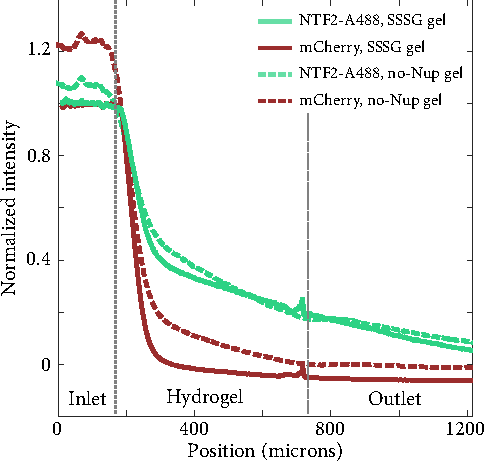
\includegraphics[width=0.4\textwidth]{figs/ch03/SSSG-control-comparison}
\label{fig:SSSG-control-comparison}
\end{SCfigure} 

\section{Pore size}

The perennial difficulty with our hydrogel nuclear pore mimics has been the pore size of the hydrogels. While hydrogels with an average pore size between 10 and 100 $\mu$m are well-studied \cite{annabi10}, as well as hydrogels with pores under 5 nm, the intermediate-porosity regime which would allow for separation of proteins in the size range 30-150 kDa (typically 5-10 nm) is difficult to reach.  We wanted to be confident that any differences in the behavior of transport factor and inert protein were due to their interactions with the Nups, not slight differences in size or interactions with the hydrogel.  At the same time, we wanted the anchored Nups to fill a significant portion of the pore.  Much of our work on hydrogel design was with the aim of achieving a suitable pore size.

To begin, there is no one mathematical definition of ``pore size'' in a hydrogel.  Several measures are used depending on the precise need.  In our case, we wanted  I tried to calculate average pore size using an equation which I will cite here.  Most people use the swelling ratio or microrheology to determine pore size, which is difficult for us because the hydrogels are not very reproducible and they are also very small.  I used a paper which does not rely on those measurements, but also is probably not very accurate.  My estimate was that the average pore size in a 10\% wt PEG hydrogel is about 5 nm, which is roughly the same size as NTF2 and mCherry.  This means that we were likely seeing a lot of interactions/hindrance by the gel in the PEG gel experiments.  We were unable to lower the PEG or crosslinker concentration significantly without going below the gel point and being unable to make gels.

Hydrogel swelling in particular has been an obstacle in our search for protein-separating hydrogels.  When polymerized from a precursor solution, hydrogels are almost never in mechanical equilibrium.  They must be soaked in an aqueous solution until they have swelled and taken up enough water to reach equilibrium.  Common methods of estimating pore size rely on the swelling ratio of the gel, i.e. the ratio of the wet to dry gel weight.  However, our gels are small enough to make that method impractical, and it is unclear whether a Nup-filled hydrogel that is allowed to swell to equilibrium in buffer will have the same properties as one that is polymerized inside a confined flow chamber.  In fact, repeated but unpredictable buckling and swelling of hydrogels within the flow chambers indicates that our hydrogels do not reach mechanical equilibrium.  Despite efforts to improve the swelling ability of our hydrogels, the lack of equilibrium swelling likely contributes to the smaller-than-ideal pore size as well as inconsistency between replicate experiments.

Of the two hydrogel substrates tested, acrylamide gels appear to have a better pore size distribution than PEG gels.  Overall, 6\% w/v acyrlamide gels are more mechanically stable and yield more reproducible results than 10\% w/v PEG gels, the lowest stable percent weight PEG gel we were able to attain. Before settling on acrylamide hydrogels, we considered several alternative crosslinkers in hopes of creating more mechanically-stable PEG hydrogels that would support larger pores.  Most notably, we moved from a 1-kDa PEG dithiol linker to an 8-kDa linker.  This change did increase the pore size of the resulting PEG gel, but it was mechanically weak and required proportionately more swelling to reach equilibrium, an impossibility inside the flow chamber.  DNA oligomers, coiled-coil rationally-designed proteins, and FSFG with both terminal cysteines were also considered as crosslinkers, but none were able to support gelation \cite{brunette15,huang14}.  Therefore, we turned our attention to acrylamide hydrogels.

Figure~\ref{fig:pc-vs-mw} shows the partition coefficient of equilibrated fluorescent macromolecules as a function of molecular weight for 6\% acrylamide gels containing no Nups.  The partition coefficient is the ratio of equilibrium concentration within the hydrogel to that in the reservoir outside; a partition coefficient of 1 indicates that the macromolecule's diffusion and equilibration is not impeded at all by the presence of the gel.  Although 250 kDa dextran has a low partition coefficient, 30 kDa transport factors and fluorescent proteins have similar partition coefficients around $\gamma = 0.7$.  The partition coefficient of inert proteins decreases when Nups are tethered to the hydrogel, as they further impede diffusion and equilibration.  

\begin{SCfigure}
\caption{Equilibrium partition coefficient as a function of macromolecule molecular weight for 6\% acrylamide no-Nup hydrogels.  NTF2, mCherry and GFP were used as 30-kDa test proteins along with 70-kDa dextran-rhodamine and 250-kDa dextran-fluorescein.\\}
\centering
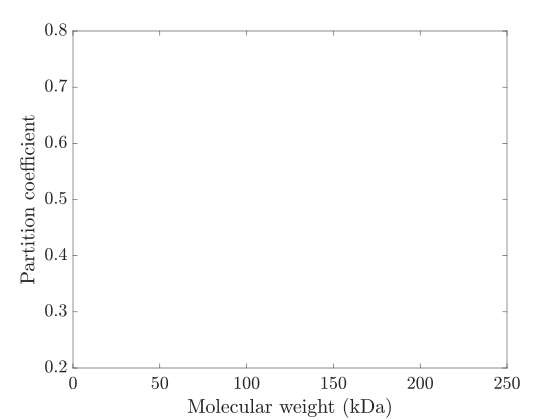
\includegraphics[width=0.5\textwidth]{figs/ch03/partition-coefficient-vs-mw}
\label{fig:pc-vs-mw}
\end{SCfigure} 

The no-Nup hydrogel dataset used in Chapter~\ref{ch:bound-diffusion}, containing 17 experiments in total, provides another measurement of partition coefficient and diffusion.  Both the NTF2 and mCherry partition coefficients are equal to 0.48 $\pm$ 0.03, statistically indistinguishable.  On the other hand, the mean diffusion constant of NTF2 was 59 $\pm$ 5 $\mu$m$^2$/s, as opposed to 44 $\pm$ 4 $\mu$m$^2$/s for mCherry.  The two values are significantly different at $p=0.02$ using a two-tailed t-test.  These results indicate that NTF2 and mCherry do not behave identically within the hydrogel, but that they equilibrate to similar values, suggesting overall a small interaction with the hydrogel scaffold.  We deemed this to be acceptable for the NTF2-mCherry pair but were not comfortable comparing the diffusion of larger proteins using acrylamide gels.
%
%\begin{table}[b!]
%\centering
%  \caption{Library of FG Nup fragments.}
%    \label{table:Nups}
%    \begin{tabular}{p{3.5cm}p{1cm}p{3cm}p{3cm}}
%      Hydrogel type & N & $\gamma_\mathrm{NTF2}$ & $\gamma_\mathrm{mCherry}$ \\
%      \hline
%No Nups* & 17 & $0.48\pm0.03$ & $0.48\pm0.03$ \\
%FSFG concat-1 & 9 & 
%
%    \end{tabular}
%\end{table}

\section{Porogens}

Given the difficulties of increasing the average pore size by changing the hydrogel composition, we investigated the possibility of introducing a porogen into the precursor solution.  To be useful, the porogen would need to be a macromolecule or particle 10-100 nm in diameter that could be evenly distributed throughout the precursor solution and then hydrogel without disrupting polymerization.  The porogen would then be digested, dissolved, or otherwise removed from the hydrogel, as it would be too large to passively diffuse from the gel on a reasonable timescale.  The pores left behind would then increase the overall pore size of the gel as well as potentially allowing the hydrogel network to swell to equilibrium even while confined in a chamber.

Two possible porogens were tried: Alginate nanospheres and high-molecular-weight dextran.  Alginate can be polymerized and depolymerized through the addition or removal of calcium ions, and dextran can be digested by dextranase.  Although both showed promise, neither was ultimately well-suited to increasing a hydrogel's pore size.

\subsection{Alginate nanospheres}
% LKM book 5, pgs 26-36
\begin{figure}
\caption{Alginate crosslinking from \cite{bruchet15}.  (A) Alginate is composed of alternating guluronate (G) and mannuronate (M) blocks.  Addition of calcium ions leads to an ``egg-box'' crosslinked structure. Calcium alginate nanospheres are coated with poly-L-lysine \cite{de03}.  (B) Alginate nanospheres should act as a porogen when added to a hydrogel precursor solution.  Removal of the spheres with EDTA should leave larger pores in the crosslinked hydrogel.}
\centering
\includegraphics[width=\textwidth]{figs/ch03/alginate-cartoon2}
\label{fig:alginate}
\end{figure}

Alginate is a polysaccharide derived from algae which polymerizes upon addition of calcium ions (Fig.~\ref{fig:alginate} (A)).  It can be depolymerized by adding EDTA or another chelator to remove the calcium.  Alginate salts are available in a number of molecular weights and viscosities, making it a promising candidate for a porogen.  If alginate nanospheres could be polymerized and added to the hydrogel precursor solution, they could later be removed with EDTA, leaving larger pores than would otherwise be present (Fig.~\ref{fig:alginate} (B)).

A number of protocols exist for creating alginate microspheres, but fewer are appropriate for nanospheres, which is the scale that we would need in order to use them as a porogen.  I made nanospheres following the method described in \cite{de03}.

I prepared 10 mL of 0.6 mg/mL alginic acid sodium salt (Sigma, low-viscosity, product number A0628) in water.  Even a small amount of sodium alginate added to water creates a viscous solution that takes a lot of time and stirring to dissolve.  I used the Garcea lab sonicator with the microtip at 40\% amplitude to sonicate the sodium alginate solution while adding 2 mL of 0.67 mg/mL calcium chloride in water drop-by-drop.  I then stirred the solution on a magnetic stir plate for 30 minutes before adding 2 mL of 0.3 mg/mL poly-L-lysine in water.  The solution was stirred 30 more minutes before finally being spun down (check spinning conditions in lab book).

I tested several methods of preparing the nanospheres for addition to the hydrogel precursor solution.  First, the nanospheres were left in the solution in which they were made.  Second, the nanospheres were spun down out of that solution at 14400g for 10 minutes and immediately resuspended in deionized water.  (The pellet becomes more difficult to resuspend if it is not immediately resuspended.) Finally, the nanospheres were lyophilized and resuspended in water.  The resuspended solution remained cloudy even after several days, and so I didn't pursue lyophilizing the nanospheres.

The radius and diffusion coefficients of the both the non-spun and spun nanospheres were determined using a Titan DynaPro dynamic light scattering (DLS) system.  The non-spun nanospheres had an average radius of 170 $\pm$ 10 nm, with an estimated diffusion constant of 1.1~$\pm$~0.1~$\mu$m$^2$/s.  The nanospheres that had been spun and resuspended had two populations: almost entirely particles of radius 210~$\pm$~10~nm and diffusion constant 1.05~$\pm$~0.06~$\mu$m$^2$/s, and a small number of very large particles.  The large particles are probably aggregates from centrifugation.

After measuring the size distribution of the two samples, I added EDTA in an effort to depolymerize the nanospheres.  The maximum final EDTA concentration was 25~mM, and the samples were left to sit up to 30 minutes.  Re-running the DLS data gave inconclusive results as to the presence or size of remaining particles.  The fits did not change much, although the large aggregates appeared to have vanished from the spun sample.  It appeared that at least some nanospheres remained.

Next, the nanospheres were added to hydrogel precursor solution, which was then crosslinked.  Several nanosphere concentrations were tested before a condition was found in which the nanospheres appeared by eye to resuspend.  An approximately 2 $\mu$L nanosphere pellet (spun down from 10 mL of solution) was resuspended in a final concentration of 0.11 mg/mL PEG-ene, 0.09 mg/mL 8K PEG dithiol linker, and 5 mM LAP, all in 50 mM MOPS buffer pH 7.4.  The MOPS buffer was chosen because it has no divalent cations (and thus will not interfere with the alginate nanospheres).  The isoelectric point of poly-L-lysine is at about pH 5, and the nanospheres should be kept above that pH so their coating remains intact.

However, even these gels were clearly inhomogeneous under 4x magnification.  In an attempt to depolymerize the nanospheres, the resulting hydrogels were rinsed with PTB pH 5 (to remove any possible poly-L-lysine coating) and then soaked in 100~mM EDTA for two days.  No change was observed under 4x magnification.  For comparison, a macroscopic alginate droplet dissolved after 20 minutes in 100 mM EDTA and vortexing.  New gels were made and soaked in a pH 5 buffer (to remove any poly-L-lysine coating) and then in a solution containing 100 mM EDTA and 200 mM sodium citrate.  Gels remained cloudy and no change was observed.

Given the difficulty in resuspending and depolymerizing the alginate nanospheres, our focus shifted to developing a dextran/dextranase porogen system.

\subsection{Dextran/dextranase porogen system}
% First proof of concept: LKM book 5 pgs. 37-47
% add diagram of porogen process + molecular structure of dextran, dextranase?
Following the alginate nanospheres attempt, we tried creating nanopores using high-molecular-weight (high-MW) dextran.  Dextran is a branched, inert polymer that is commerically available at molecular weights up to 250 kD.  We used two sizes as porogens, 70 kD ($R_H \approx 10$ nm) and 250 kD ($R_H \approx 15$ nm) \cite{masuelli13}.  

As a proof of concept, I made and crosslinked precursor solutions containing 100~$\mu$M 70~kD dextran-rhodamine or 250~kD dextran-fluorescein.  The precursor contained 12\% acrylamide and 3.3\% bisacrylamide in 50~mM sodium acetate (NaOAc) buffer pH~5 as well as 2~mM LAP.  The precursor solution was crosslinked as 1-$\mu$L hydrogels in a 400-$\mu$m tall PDMS gasket chamber for 20~s using the UV LED.  After rinsing with NaOAc buffer, the chamber was filled with a freshly-made solution of 20~mg/mL dextranase (Sigma, D5884, dextranase from \textit{Penicillium sp.}) in NaOAc buffer.  Chamber was immediately placed in the Olympus widefield's environmental chamber, held at 37$^\circ$C, and imaged overnight. The fluorescence intensity in the dextranase-treated gels decreased significantly more rapidly than that of gels which contained dextran but were not treated with dextranase (Fig.~\ref{fig:dxase-equilibration}).  In the case of 70~kD dextran, the fluorescence reached a steady value (equilibrated, same as that in the reservoir) in approximately 100 minutes, while the non-treated case wasn't equilibrated after an overnight incubation.  For the 250~kD dextran, both the treated and non-treated gels reached an equilibrium in approximately the same amount of time, but the treated gel equilibrated much closer to the reservoir level than the non-treated gel.  Both sets of gels indicate that dextranase is able to digest the dextran within the hydrogels, allowing a significant amount of dextran and digest products to leave the gel, as expected.
\begin{SCfigure}
\caption{Exit of fluorescent dextran from hydrogels after digestion with dextranase.  Each hydrogel originally contained 100 $\mu$M dextran and was treated with 20 mg/mL dextranase as described in the text.  The total fluorescence intensity within the gel was monitored as a function of time as it approached equilibrium with the buffer in the reservoir.  Intensity was normalized to intial gel fluorescence.}
\centering
\includegraphics[width=0.7\textwidth]{figs/ch03/dxase-equilibration}
\label{fig:dxase-equilibration}
\end{SCfigure}
% dextranase gels from 1/24/18; control gels from 1/22/18
% I also seem to have a replicate from 3/6/18

The next step in attempting this porogen system was recreating the effect in FSFG gels.  Unfortunately, it became clear that the dextranase was digesting the FSFG as well as the dextran (Fig.~\ref{fig:dxase-FSFG}).  
\begin{SCfigure} % gel is from 6/19/18
\caption{SDS-PAGE gel demonstrating dextranase digestion of FSFG.  Three conditions are shown, with and without dextranase: precursor solution with FSFG, FSFG only, and precursor with FSFG and dextran.  In each case, addition of dextranase destroys the FSFG band at 15 kDa and produces bands of smaller degradation products.  Dextranase alone is shown for reference.  AnyKd PAGE gel (BioRad), 100 V, 80 minutes.\\}
\centering
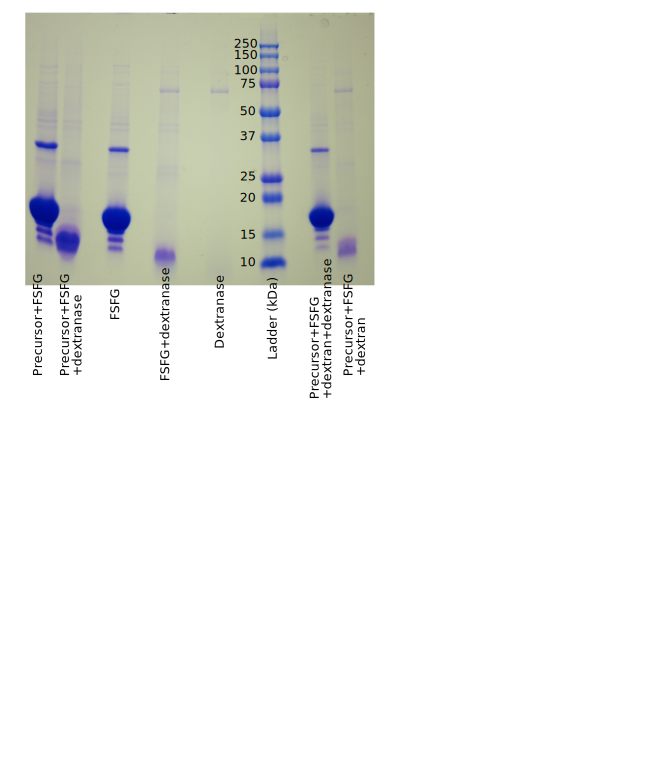
\includegraphics[width=0.5\textwidth]{figs/ch03/FSFG+dxase_PAGE}
\label{fig:dxase-FSFG}
\end{SCfigure}
 At this point, we stopped trying to use the dextran-dextranase porogen system for FSFG gels.  However, we did investigate the effect of dextran-dextranase treatment on the pore size in acrylamide hydrogels without anchored proteins.  Contrary to expectations, dextran-dextranase treatment did not increase subsequent diffusion of fluorescent proteins into the treated hydrogels.  For these experiments, I used 200~kD non-fluorescent dextran in the acrylamide precursor solution.  After the gels (either 12\% or 6\% final acrylamide concentration) were crosslinked, I treated them with 20~mg/mL dextranase solution in sodium acetate buffer (freshly made solution) for 2 hours at 37$^\circ$C in an incubator.  Then I rinsed the gels with buffer and let them sit in fresh buffer in the fridge overnight.  (Check this - sometimes I used a syringe pump to flow 10~mL of PTB through overnight, instead of letting the chamber sit.) The next day, I challenged the gels with a solution containing 10~$\mu$M each IgG-Alexa488 (150~kD) and mCherry (28~kD).  I monitored the accumulation of each protein in the gel over time (Fig.~\ref{fig:dxase-results}).  In both the 12\% and 6\% acrylamide gels, dextran-dextranase treatment did not improve influx of IgG-Alexa488 over corresponding non-treated gels.  In 6\% acrylamide gels, the influx of mCherry also remained approximately the same for treated and non-treated gels.  This indicates that dextran-dextranase treatment does not significantly increase the pore size in acrylamide hydrogels.  This is probably because significant dextran remains in the gel even after dextranase treatment, as suggested by Fig.~\ref{fig:dxase-equilibration}.
\begin{SCfigure}
\caption{Comparison of protein accumulation within hydrogels made with or without dextran.  Reservoirs contained 10 $\mu$M IgG-A488 and mCherry. (A) Accumulation in a 12\% acrylamide hydrogel containing no Nups or dextran. (B) Accumulation in a 12\% acrylamide hydrogel containing no Nups but made with 15\% w/v 200 kDa dextran and digested for 2 hours at 37$^\circ$C with 20 mg/mL dextranase.}
\centering
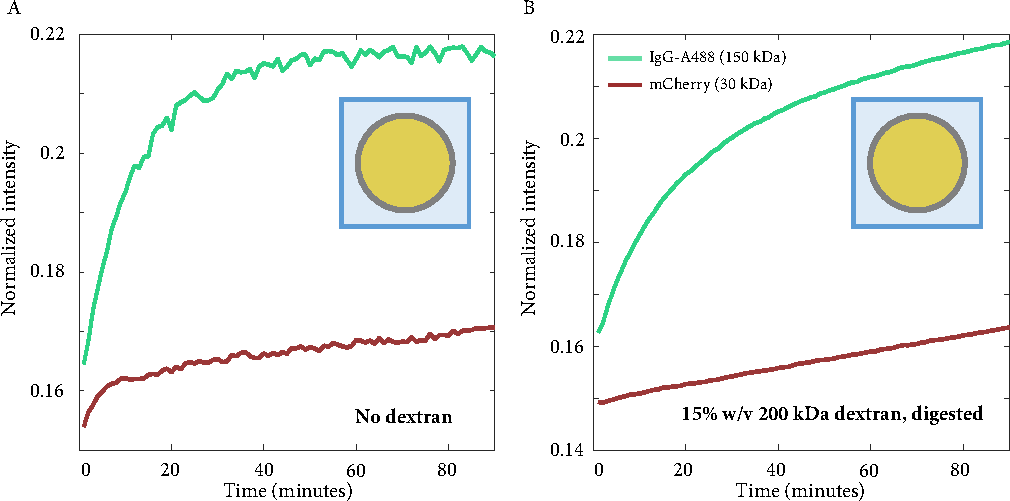
\includegraphics[width=0.7\textwidth]{figs/ch03/dxase-results}
\label{fig:dxase-results}
\end{SCfigure} %a - 2018-10-9_1 (no nups, no dx, 12% ac), b = 2018-10-9_2 (no nups, 15% dx 200 kD, dxase treated, 12% ac)
%Unusually, the 12\% acrylamide gels showed an odd effect with mCherry accumulation.  In two separate instances, dextranase treatment appeared to suppress the entry of mCherry into both the dextran-containing hydrogel and the no-dextran control gel in the same chamber (Fig.~{fig:mCherry-suppression}).  IgG-Alexa488 accumulation remained the same as a non-treated gel.  Tests of gels without dextran but treated with dextranase did not show this mCherry suppression.  I didn't thoroughly investigate this effect.  The only thing I can think of that's different between the gels that did and didn't show mCherry suppression is that the gels that suppressed mCherry were in the presence of both dextran and dextranase, and therefore also dextran digestion products (which are mostly maltose, I believe).  Maybe the presence of maltose (despite the fact that it should have been thoroughly rinsed away) interfered with the accumulation of mCherry.  It's odd.
%\begin{figure}
%\caption{Suppression of mCherry in control gels that were in the presence of dextranase, dextran, and dextran digestion products (maltose).}
%\centering
%\includegraphics[width=\textwidth]{figs/ch03/mCherry-suppression}
%\label{fig:mCherry-suppression}
%\end{figure}

In conclusion, dextranase is capable of digesting a significant fraction of high-MW dextran within an acrylamide hydrogel.  However, a significant amount of the dextran still remains in the gel even after an overnight rinse, meaning that dextran-dextranase treatment does not result in noticeably larger pores overall.  In addition, the dextranase we used digested the FSFG peptide as well as dextran.  Dextran-dextranase treatment is not suitable as a porogen system for our hydrogels.

\section{Polymerization using confocal microscope}
\label{sec:confocal-crosslinking}

Given the problems that arose using photomasks and a UV LED to make hydrogels, we tested a crosslinking method using a 405 nm laser on the Nikon A1R spinning disc confocal microscope in the JSCBB microscopy facility.  Once a region of interest has been defined with the Nikon software, the photobleaching setting can be used to selectively expose regions of the field of view to UV light.  The precursor solution therefore crosslinks in the region of interest only.  This method is similar to that used in \cite{paustian13}, but the masking is done using the A1R software instead of a physical mask in the back focal plane.

We were able to ``draw'' hydrogels of arbitrary shapes using the 10x objective on the confocal along with the 405 nm laser at 100\% power.  Figure~\ref{fig:LW-gel-images} shows hollow rings with an outer diameter of about 600 $\mu$m and an inner diameter of 500 $\mu$m, as well as lines with a width of about 50 $\mu$m.  In order to crosslink the precursor solution, two raster-scans of the laser across the region of interest were needed, with the longest-allowable dwell time per pixel.  (In the microscope settings, the shortest dwell time is set as `1' and the longest as `1/32'.)  The precursor solution contained 0.5 mM LAP, 110 mg/mL 20kD 8-armed PEG-norbornene, 11 mg/mL 1kD PEG-dithiol, and 1 mM TCEP in PTB; it was used to fill 70-$\mu$m-thick sticky-tape or NOA flow chambers.

% hydrogel recipes on LKM book 4 pg 47, 56

Crosslinking with the confocal has several advantages over LED crosslinking.  Significantly smaller features are possible using the confocal.  50-$\mu$m features are consistent and reproducible, and features down to approximately 25 $\mu$m are possible, in contrast with the effective 100-$\mu$m lower limit using the LED and photomasks.  Additionally, arbitrary shapes, including shapes with inner cavities, are possible using the confocal.  Multiple small hydrogels can be created in the same chamber, including hydrogels of varying composition, created by removing the excess precursor solution and refilling the chamber with a different solution.  Finally, the degree of crosslinking can potentially be varied by changing the photobleaching settings.

\begin{SCfigure} % LKM book 4 pg 81 9/6/16 (rings), LKM book 4 pg 77 8/25/16 (lines)
\caption{Image of laser-written hydrogels. (A) Ring hydrogels containing no Nups.  Reservoir contains 20 $\mu$M NTF2-A488 and mCherry. (B) Line hydrogels containing FSFG-A647. Reservoir contains precursor solution with FSFG-A647. Photobleaching within gel by 405 nm laser is evident.}
\centering
%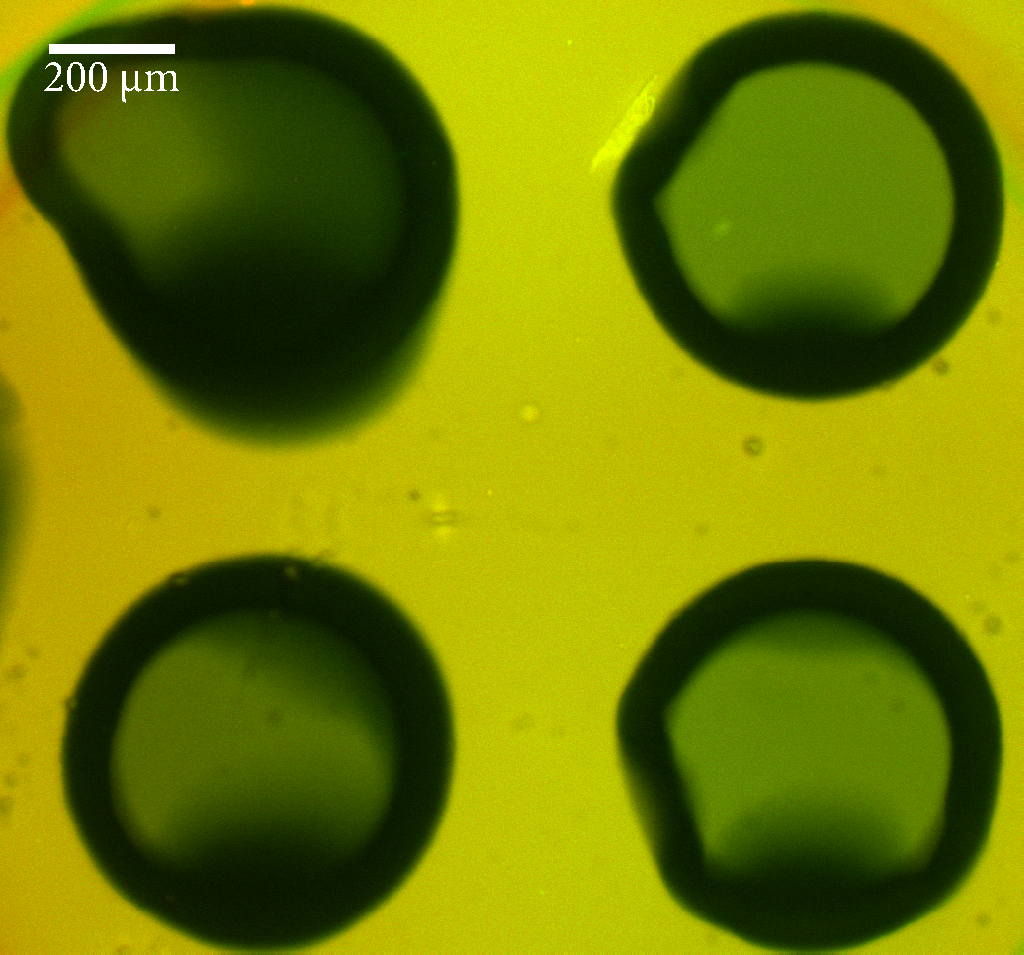
\includegraphics[width=0.5\textwidth]{figs/ch03/160906_laserGelImage_200umscale.pdf}
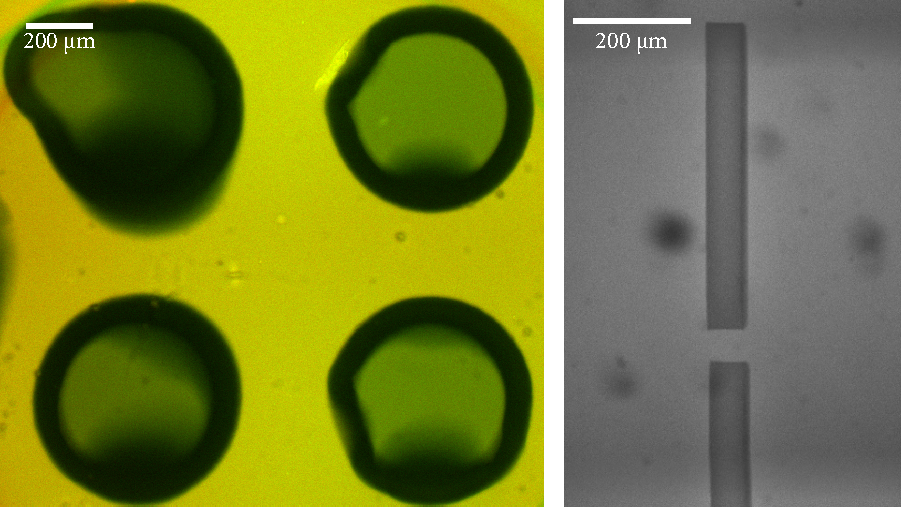
\includegraphics[width=0.7\textwidth]{figs/ch03/example-LW-gels}
\label{fig:LW-gel-images}
\end{SCfigure} % microscope settings for rings: 1/32 dwell, 2 loops, 100% photobleaching intensity, nominal outer diameter = 600 um, nominal inner diameter = 500 um

The most appealing geometry made possible with confocal crosslinking is the hydrogel ring, as shown in Figs.~\ref{fig:LW-gel-images} and \ref{fig:LW-NTF2-images}.  Unlike all other hydrogel-chamber geometries, the inner reservoir is small enough to equilibrate in only a few hours (Fig.~\ref{fig:ring-acc-and-profile}).  Ideally, the hydrogel rings could have been used to test selective flux through the NPC mimics, a possibility not offered by other hydrogel-chamber geometries, which are optimized for testing influx into the hydrogels only.  Long thin lines can also be written with the confocal by repeatedly moving the field of view and re-crosslinking, overlapping the new segment with the previous.  This geometry could be useful in creating counter-propagating flow chambers with hydrogel windows.

\begin{SCfigure} % LKM book 4 pg 65
  \centering
  \caption{Sample (A) accumulation and (B) intensity profile plots for a 50 $\mu$m thick confocal-crosslinked ring nominally containing 10 mg/mL FSFG. Intensity normalized to inlet reservoir.  Inlet contains 25 $\mu$M NTF2-Alexa488 and mCherry in PTB.\\}
  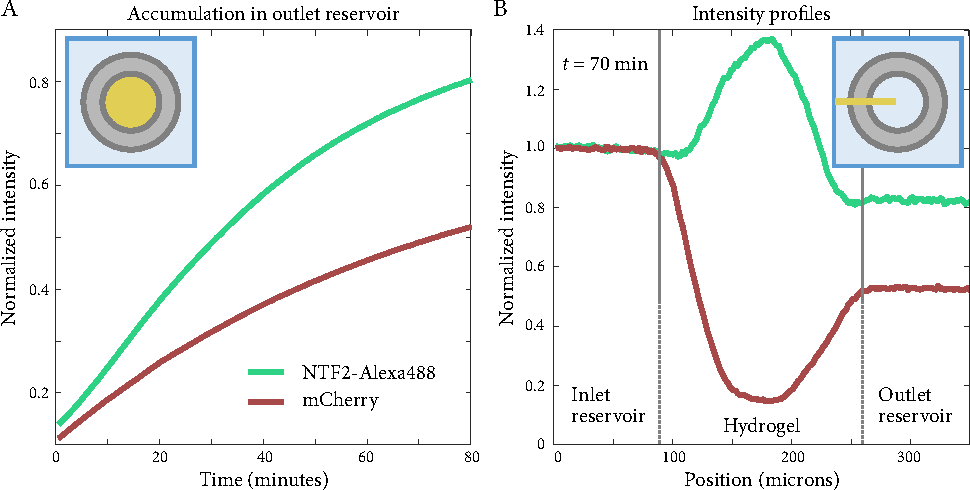
\includegraphics[width=0.7\textwidth]{figs/ch03/ring-acc-and-profile}
\label{fig:ring-acc-and-profile}
\end{SCfigure} %16-08-19, chamber 1, #2 (1/32 dwell time, 2 loops) 

Confocal crosslinking does not damage FSFG, as demonstrated in Fig.~\ref{fig:LW-NTF2-images}.  Hydrogels were made using the precursor solution described above with the addition of 10 mg/mL FSFG-cys.  After soaking in PTB buffer overnight, a mixture of 25 $\mu$m each NTF2-Alexa488 and mCherry was added to the outer reservoir.  After two hours of equilibration, the FSFG hydrogels showed a partition coefficient greater than one for NTF2-Alexa488 but smaller than one for mCherry.  This indicates that FSFG is anchored into the gel and that NTF2-A488 is able to bind it.

Finally, Norland Optical Adhesive (NOA) can also be crosslinked using this method.  Complicated flow chambers can be created, although it is labor-intensive and difficult to remove all of the excess NOA afterwards.

\begin{figure} % LKM book 4 pg 57 (line); NEED TO FIND RING lookup for info and scale
%laser-written line FSFG hydrogel. 8/17/16
\caption{Images of laser-written hydrogels nominally containing 10 mg/mL FSFG. Reservoirs contain 20 $\mu$M NTF2-A488 and mCherry. (A) Hydrogel ring, likely with lightly-crosslinked inner reservoir. (B) Hydrogel bar separating large inlet and small outlet.}
\centering
%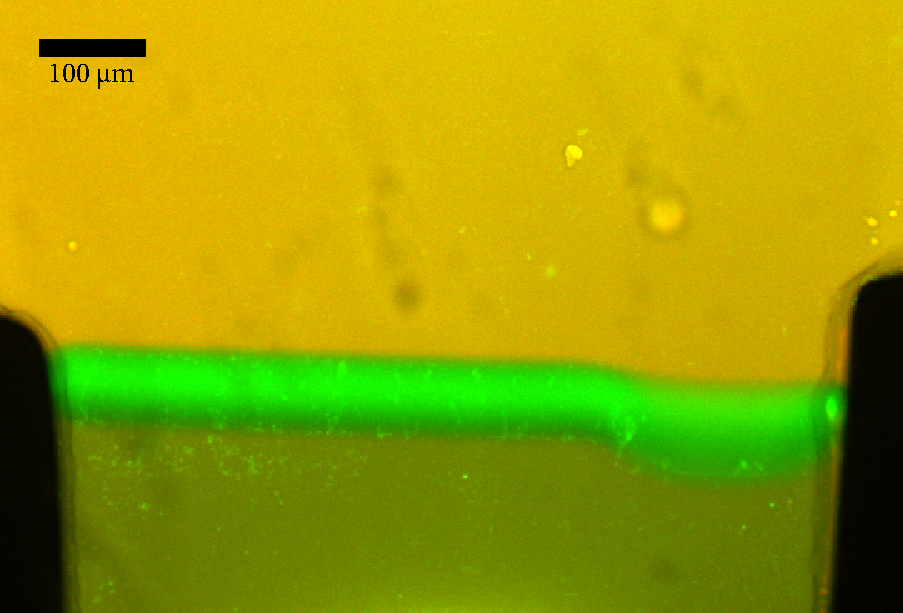
\includegraphics[width=0.5\textwidth]{figs/ch03/160817-bar-image-100umScale.pdf}
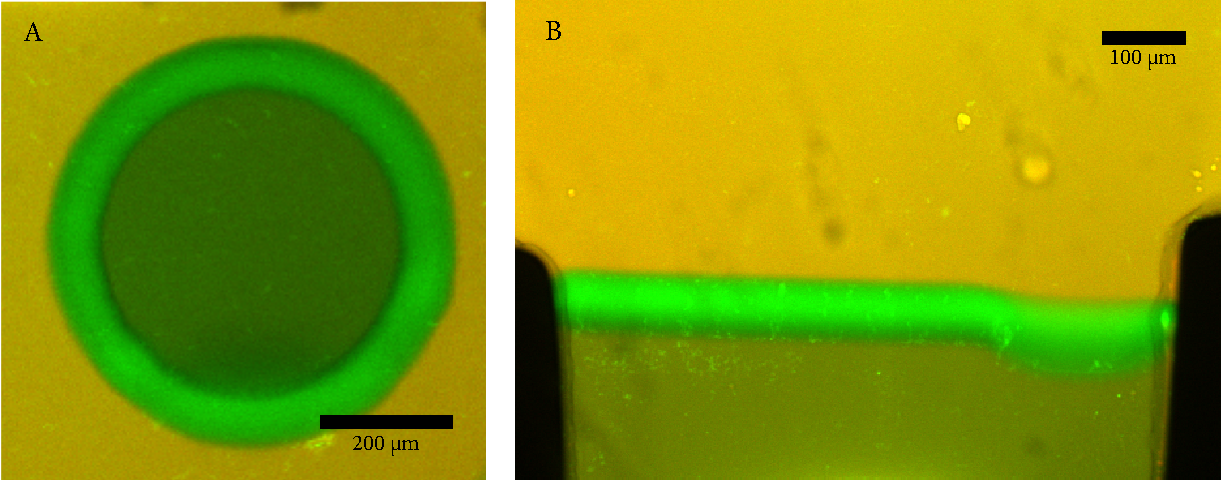
\includegraphics[width=0.8\textwidth]{figs/ch03/example-LW-gels-NTF2}
\label{fig:LW-NTF2-images}
\end{figure} % microscope settings for bar: 1/32 dwell, 2 loops, 100% photobleaching intensity, nominal thickness 50um, nominal concentration 50 mg/mL FSFG (slightly unclear? could be 10), 25 uM each NTF2-A488 and mCherry
% I am confused as to the date of the bar image.  Saved as 160817 in the microscopy folder so that's probably right

Despite the advantages of confocal crosslinking, several obstacles combined to ultimately make this method unusable for our purposes.  The most serious problem was that of stray crosslinking.  Areas outside of the defined region of interest were often unpredictably crosslinked, as can be seen in Fig.~\ref{fig:LW-gel-images}.  Stray crosslinking outside of the rings is limited by rinsing the gels within 5 minutes of crosslinking, removing any excess precursor solution \cite{paustian13}.  However, rinsing the chamber does not remove precursor solution from the ring's inner reservoir.  Stray crosslinking in this reservoir is often more difficult to detect and more damaging to the experimental results. Figure~\ref{fig:LW-NTF2-images} illustrates the problem: the ring has been equilibrated with NTF2-A488, which has preferentially entered the inner reservoir over mCherry.  The concentration of NTF2-A488 is, in fact, higher in the inner than the outer reservoir, indicating that there is some low concentration of FSFG available in the inner reservoir for binding to NTF2.  As the hydrogel was soaked in buffer overnight after crosslinking, any mobile FSFG remaining from the precursor solution has been removed, meaning that the remaining FSFG is most likely anchored into a lightly-crosslinked hydrogel that fills the inner reservoir.  The presence of this gel alters the results of an equilibration experiment by artificially increasing the final NTF2 concentration in the inner reservoir.

With help from Danielle Konetski and Christopher Bowman, we attempted to address the stray crosslinking by adding a photoinhibitor to the precursor solution.  The radical inhibitor 2,2,6,6-tetramethylpiperidine 1-oxyl (TEMPO) can be used in aqueous solution to limit crosslinking \cite{chatani14}.  We tested the effect of the photoinhibitor using a precursor solution as described above with the addition of 0.5 mM TEMPO.  While the edges of the resulting hydrogels became marginally sharper, stray crosslinking was still evident, especially in the inner reservoir.

%Help from Dani Konetski in Bowman lab with TEMPO and digital light projector (didn't work)
% TEMPO - LKM book 4 pgs 83-93

Another significant problem was swelling and buckling of the hydrogels.  Despite the hope that thinner hydrogels would swell and equilibrate more easily, buckling of the rings and lines was pervasive and difficult to predict (Fig.~\ref{fig:LW-gel-images}).  Ring hydrogels in particular often developed minor leaks due to buckling.  Despite a great many attempts to improve the swelling problem (see various other sections), the rings ultimately could not be used for selective transport experiments.

\begin{SCfigure} % LKM book 4 pg 60
\caption{Effect of dwell time and loop number on edge-dip effect in equilibrated, confocal-crosslinked ring hydrogels.  Nominal FSFG concentration is 10 mg/mL.  Reservoirs contain 20 $mu$M NTF2-A488 and mCherry in PTB.  Intensity profiles are shown for a hydrogel polymerized with $t_\mathrm{dwell} = 1/32$ and two loops (solid lines) and a hydrogel polymerized with $t_\mathrm{dwell} = 1$ and 64 loops. \\}
\centering
\includegraphics[width=0.62\textwidth]{figs/ch03/dwell-time-effect}
\label{fig:dwell-time-effect}
\end{SCfigure} %16-08-19, chamber 1, #2 (1/32 dwell time, 2 loops) compared to #6 (1 dwell time, 64 loops)

One interesting feature of confocal crosslinking is the degree of control it affords over the illumination method.  In the A1R's photobleaching mode, the 405 nm laser is raster-scanned over each pixel in the field of view.  The shutter is toggled in order to illuminate only pixels within the predefined region of interest.  The controls permit the laser intensity, dwell time at each pixel, and number of raster scan loops to be varied.  The laser intensity was always kept at 100\%, but changing the dwell time and loop number had a dramatic effect on the final properties of the hydrogel.

Generally speaking, a longer dwell time at each pixel and a low number of loops gave the best results.  (See if I can try to get dwell times in absolute time instead of fold change.)  Figure~\ref{fig:dwell-time-effect} shows post-equilibration profiles for two hydrogel rings made with different illumination settings.  Each gel received the same total illumination time, but in one case the dwell time was reduced 32-fold and the loop number increased by the same factor.  In both cases, the hydrogels were soaked in PTB buffer overnight and then challenged with 25 $\mu$M NTF2-Alexa488 and mCherry.  After 70 minutes, sufficient NTF2 had accumulated in the gel to make the differences between gels obvious.  The low-dwell-time hydrogel accumulated less NTF2 and displayed noticeable dips in NTF2 accumulation at both its inner and outer edges.  The edge-dip is reminiscent of those noted in the gels crosslinked by photomasking and the UV LED.  While the cause of the dip is unclear, it may be the result of diffusion of fresh precursor solution into the edge region over the course of the crosslinking process.  The fresh precursor then crosslinks, leading to a dense hydrogel edge that excludes NTF2 and mCherry.  This hypothesis is consistent with the observation that a longer dwell time and fewer raster loops largely eliminated the edge dip.  With fewer raster loops, there is less opportunity for diffusion of uncrosslinked precursor solution into the gel edge.  It should also be noted that the edge dip does not form when an entire droplet of precursor solution is crosslinked with the UV LED (i.e. no mask is used), further supporting the diffusion explanation.  In any case, long dwell times and low loop numbers are clearly preferable with confocal crosslinking.

In conclusion, confocal crosslinking has a number of advantages over LED crosslinking, and a corresponding number of obstacles.  Despite the attraction of testing selective transport using small hydrogel rings, we ultimately chose to use a much simpler hydrogel geometry and crosslinking method.

\section{Transport factor constructs}

A wide variety of transport factors exist, specialized for the import and export of particular cargo.  Almost all protein separation experiments we performed made use of Nuclear Transport Factor 2 (NTF2).  This transport factor is relatively small (28 kDa dimer) and, unlike most other transport factors, does not require active release of cargo after transport. NTF2 transports RanGDP as part of a mechanism which maintains a high RanGTP concentration in the nucleus, necessary for the active release of other protein cargos \cite{ribbeck98}.  The choice to focus on NTF2 was made for a number of reasons: the lack of facilitated release makes it a simple first choice to study, it is small enough to move reasonably quickly through hydrogels, and it is readily expressed in bacteria and purified.

His-tagged yeast NTF2 in the Kan-resistant plasmid pRSF was expressed in BL21 DE3 Gold cells and purified using the procedure described in Appendix~\ref{appx:protein-purification}.  When necessary, NTF2 was covalently labeled with fluorescent dyes as described in Appendix~\ref{appx:dye-labeling}.  In addition to wild-type yeast NTF2, several variants were created in order to address shortcomings of NTF2 in the experimental setup.  In particular, efforts were made to prevent the presence of any NTF2 monomers and to eliminate the need for dye labeling.  Finally, a point mutant of NTF2 was created with the intent of disrupting the binding pocket and providing another non-binding negative control protein to complement mCherry.

Beyond NTF2, we briefly tested the influx of Kap121, a member of the well-studied karyopherin family of transport factors, into hydrogels.  Although the Kap121 and its fluorescent cargo protein clearly bound to the FSFG in the hydrogel, the pore size remained too small for significant import into the gel.

The remainder of this section provides an overview of the transport factor constructs we created.  Much of the cloning work was done by Eric Verbeke and Scott Tilden.

\subsection{Covalently-tethered NTF2 dimer}

Despite the work done to increase the hydrogel's average pore size, we often observed that NTF2 and mCherry equilibrate to different extents and on different timescales even in hydrogels containing no Nups or nonbinding Nups.  As these proteins are nominally the same size, this implies that that they may be interacting differently with the hydrogel substrate, or that they may not be the same size after all. NTF2 is a 28 kDa homodimer whose monomers are 14 kDa.  If there exists an appreciable population of NTF2 monomers within the hydrogel, these will equilibrate more rapidly and to a higher concentration than the larger mCherry.  The dissociation constant $K_D$ of mammalian NTF2 is about 1 $\mu$M \cite{chaillan-huntington01}.  Assuming this is approximately true for yeast NTF2 as well, there should be very little monomeric NTF2 present at our typical reservoir concentration of 20 $\mu$M.

However, we designed a covalently-tethered version of NTF2 to eliminate the possibility of monomerization.  This consisted of two NTF2 monomers connected by a flexible amino-acid tether (Fig.~\ref{fig:NTF2} (A)).  Several trial tethers with their length and composition are shown below:

\begin{align*}
\mathrm{10aa-linker}&:&\mathrm{TSGSGSGSPG}\\
\mathrm{15aa-linker}&:&\mathrm{TSGSPRGSSGSGSPG}\\
\mathrm{18aa-linker}&:&\mathrm{TSPGLVSRGSGSGSGSPG}
\end{align*}

Eric Verbeke and Scott Tilden successfully cloned covalently-tethered NTF2 with all three tethers.  Unfortunately, no binding was seen when the NTF2 was introduced to an FSFG hydrogel.  It is likely that the tether interferes with the binding pockets or dimerization interface. (lookup: did we get these to express?  any test?)

\subsection{NTF2-GFP}

In addition to the potential problem of NTF2 monomerization, the fluorophores that labeled NTF2 were prone to hydrolysis, leaving an unknown amount of free dye in the reservoir mixture.  Free dye is indistinguishable from labeled NTF2 in the influx and selectivity experiments, and it is important that not be present in appreciable amounts.  This problem is addressed through other means in Sec.~\ref{sec:free-dye}, but we also approached it by engineering a GFP-NTF2 fusion protein.  Such a protein would eliminate the need for dye-labeling the NTF2 and therefore eliminate free dye in the chamber entirely.  

However, as GFP is also approximately 30 kDa, the fusion protein is much larger than NTF2 alone.  To mitigate this problem, a GFP-NTF2-NTF2 version was also created (Fig.~\ref{fig:NTF2} (A)).  While this is still larger than an NTF2 dimer, it contains only one copy of GFP.  Both constructs are in the pET21 plasmid, his-tagged, and expressed in BL21-DE3 Gold cells.  They were purified using a cobalt affinity column in PTB and 1:1000 PIC and eluted with 250 mM imidazole, yielding ample protein with moderate degradation products.

Figure~\ref{fig:NTF2} (B) and (C) show that neither construct is able to bind to FSFG hydrogels.  Again, the binding pockets or dimerization interface may be disrupted by the tethers, or the fusion protein may simply be too large.

\begin{figure} % LKM book 4 pg 60 % GFP-NTF2 = 150917, GFP-NTF2x2 = 150928
\caption{Cartoon of various NTF2 constructs}
\centering
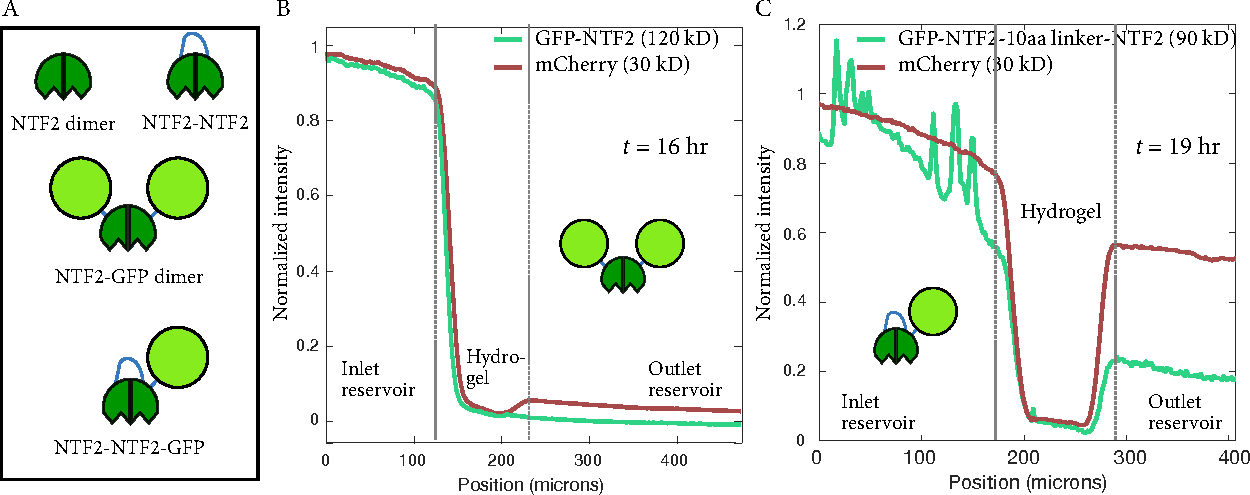
\includegraphics[width=\textwidth]{figs/ch03/NTF2-constructs}
\label{fig:NTF2}
\end{figure}

\subsection{Non-binding NTF2 F5R}

Although mCherry is a similar size as the NTF2 dimer and makes an acceptable negative-control inert protein, it may well interact differently with the hydrogel scaffold than NTF2 does.  A better control would be a non-binding mutant form of NTF2.  (lookup: I wrote my reasoning for the F5R mutant in a lab book, I'm pretty sure) A W7A point mutant in mammalian NTF2 reduced its affinity for FG Nups \cite{bayliss99}.  A corresponding mutant in yeast NTF2 is F5R.  This mutant was cloned, expressed, and purified. (lookup: who did most of the work?)  Further tests, such as NMR, are needed to verify its binding affinity for FSFG.

\subsection{Kap121 and NLS-GFP}
% Kap121 growth and purification - LKM book 2 pg 79, LKM book 3 pg 13, Chris Lawton book 1 pg 65, Loren's protocols in Google Drive, Jackie's paper
The karyopherins (Kaps) are a canonical class of transport factors.  They transport proteins tagged with nuclear localization signals (NLS) through the nuclear pore.  We were interested in testing Kaps because they are widely studied and much larger than NTF2, so selective transport would be more apparent.  Eric Verbeke engineered two GFP-NLS constructs: GFP-Spo12 and GFP-Pho4.  These constructs were his-tagged, inserted into pET21b, expressed in BL21-DE3 Gold cells, and purified using a cobalt affinity column. 
% GFP-NLS LKM book 2 pg 133
Kap121-GST was expressed and purified following \cite{tetenbaum-novatt12} and the GST subsequently cleaved with thrombin resin (Fig.~\ref{fig:Kap121}~a).
\begin{figure} % LKM book 4 pg 60
\caption{SDS-PAGE showing Kap121 purification (purified by Chris Lawton), picture of influx, intensity profiles}
\centering
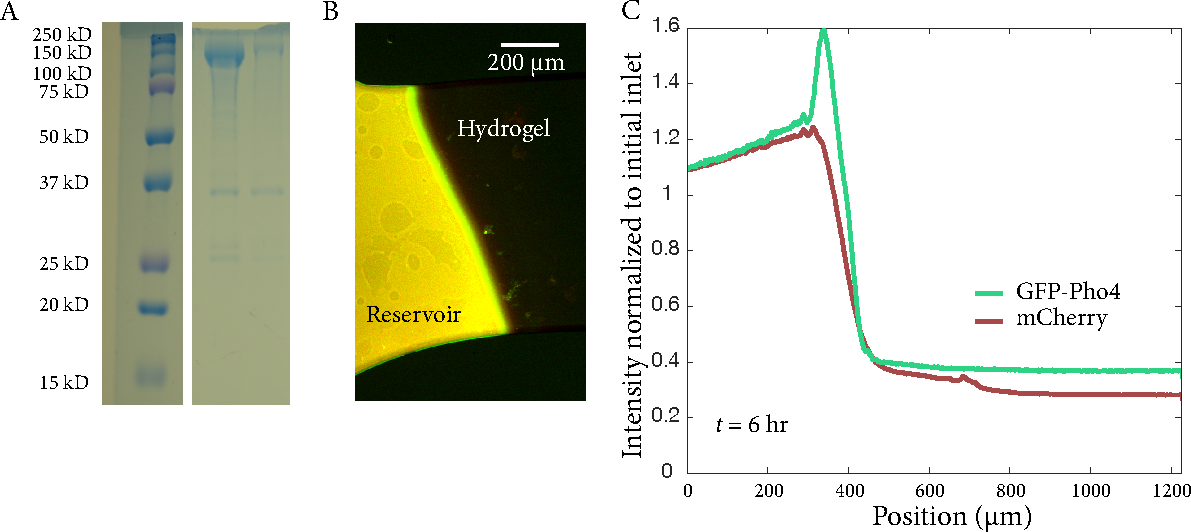
\includegraphics[width=0.8\textwidth]{figs/ch03/Kap121}
\label{fig:Kap121}
\end{figure} % 12 polyacrylamide gel, 2hr, 100V, 10uL samples, purified by Chris Lawton, 5/28/15, saved in Laura's folder on lab desktop

% microscopy of Kap121 and Pho4 on 150602, LKM book 3 pg 19, used final frame of Kap121_Pho4 03 movie

Kap121 binding and influx was tested using a hydrogel made from precursor solution containing 0.05 wt\% Irgacure2959, 110 mg/mL 20kD 8-armed PEG-norbornene, 11 mg/mL 1kD PEG-dithiol, and 1 mM TCEP in PTB, crosslinked for 2 minutes under the UV LED.  After soaking in PTB overnight, 5 $\mu$M Kap121, 10 $\mu$M GFP-Pho4, and 100 $\mu$M mCherry in PTB were added to the inlet reservoir.  Selective influx of the Kap121/GFP-Pho4 complex was evident, since the complex accumulated at the edge of the hydrogel (Fig.~\ref{fig:Kap121}~b and~c).  The bright band demonstrates binding of FSFG to Kap121 as well as of Kap121 to GFP-Pho4.  Over the course of several hours, the GFP front remained localized at the edge of the gel, likely indicating that the pore size of the hydrogel was too small to accomodate the Kap121/GFP-Pho4 complex.  Given the large size of this complex, the pore size was never increased sufficiently for influx into the hydrogels.

 % same as 110 mg/mL 20kD 8-armed PEG-norbornene, 11 mg/mL 1kD PEG-dithiol, and 1 mM TCEP in PTB;
%same as 10 wt% PEG, 0.5 thiol:ene ratio (LKM book 2 pg 73)

\section{Dye-labeling and free dye}
\label{sec:free-dye}
% matlab results are saved in /Volumes/houghgrp/Old Processed Images/Old Analysis/FSFG dataset/exponent-fits.mat
Figures
\begin{enumerate}
\item Typhoon image of dye, Matlab peaks
\item Example of single- and double- exponential fits
\item goodness of fit measurements for single- and double- exponential fits
\end{enumerate}
We have to label NTF2 with a fluorescent dye to use it as a test transport factor.  For the most part, we've used Alexa Fluor 488 as the dye.  (Most recently we switched to fluorescein because it's easier to photobleach.)  There are several choices of labeling chemistry.  We've used both NHS and SDP esters, which label the exposed lysines of NTF2, of which there are several.  We've also tried using Alexa488-maleimide to label the cysteine of an engineered NTF2-cys.  Both labeling chemistries result in bonds that eventually hydrolyze, cleaving the dye from the protein.  This is a major problem for the experiments, since free dye (about 1kD) diffuses much faster than dye bound to a protein and is experimentally identical.  Non-negligible levels of free dye would give the impression that NTF2 is equilibrating significantly faster than it actually is.  The maleimide-labeling chemistry is more stable, but in practice not as efficient as the ester-labeling protocol.  It also requires using NTF2-cys, which could introduce other issues.  Mostly I stuck with the lysine-labeling protocol, which needed significant optimization to minimize free dye issues.  Eric did a lot of work in optimizing the cysteine-labeling protocol, and I took his work as a base in optimizing the lysine-labeling protocol.

The major change is the increased wash step, and the immediate aliquoting and freezing before use.  I also began to be much more careful with characterizing the results of the labeling.  Immediately after finishing dialysis, I run a BCA to quantify the protein concentration in the labeled sample.  The same day, I aliquot and freeze all the protein except a sample for the remaining tests.  As soon as possible, I run a native PAGE gel, including the labeled protein sample as well as a free dye sample.  After running the gel, I image it in the Alexa488 channel using the Typhoon, and then stain with Coomassie to make sure the protein hasn't degraded.  I use Matlab to compare the amplitude of the labeled-protein band and the free-dye band that remains in the labeled-protein sample.  Typically, the free dye band is 1-3\% the amplitude of the labeled-protein band.  Finally, I measure the absorbance of the labeled protein at 494 (check this wavelength) nm and use Beer's law to find the concentration of Alexa488.  I can compare this measurement with the protein measurement from the BCA to calculate a labeling efficiency.  Include some sample efficiencies here.  I typically get lower efficiencies than other people report.  I spoke to Annette and she had no major suggestions.  In principle, doing the reaction under nitrogen would help, but Annette gets something like 90\% efficiency without doing that.  I use the labeled NTF2 immediately after thawing if possible, and no more than a week after thawing.

We also tried to make NTF2-GFP to fix the free dye problem (see section above).

In addition to the tests I run on each batch of labeled NTF2, at one point I did some mathematical analysis to confirm that the free dye was only a minor problem in the experiments I had already run.  In order to confirm that, I fit the accumulation curves to single or double exponentials (they really should have been erfc functions but I approximated.)
%%%%

If there is no free dye, as in the case of the mCherry accumulation, the accumulated intensity $I(t)$ can be approximated as
\begin{equation}
I(t) = A_1\exp(-t/\tau_1) +C
\label{eq:single-exp}
\end{equation}
with some amplitude $A_1$, equilibration lifetime $\tau_1$, and constant offset $C$.  In this case, a non-zero value of $C$ is likely due to background fluorescence.  If, on the other hand, a sample contains a population of small, free dye molecules as well as large labeled protein, both populations will equilibrate at different rates, leading to an accumulated intensity of
\begin{equation}
I(t) = A_1\exp(-t/\tau_1) + A_2\exp(-t/\tau_2)+C
\label{eq:double-exp}
\end{equation}
where each population has an equilibration lifetime as well as an amplitude related to its abundance in the sample.

I fit a collection of 43 accumulation experiments to both Eqns.~\ref{eq:single-exp} and \ref{eq:double-exp}.  I compared the resulting parameters as well as the adjusted R-square value of each fit.  Adding more parameters to the fit will always improve the fit, but the adjusted R-square is intended to account for the effect of adding more parameters to a model.  A higher adjusted R-square therefore means a better fit.

The mCherry accumulation fits did not noticeably improve when moving from the single to the double exponential.  In addition, the lifetimes and amplitudes of each component of the two-component fit were apparently uncorrelated.  Both results support the fact that there is no free dye in the red channel, since the only fluorescence is coming from mCherry.

On the other hand, the NTF2 fits did result in a higher adjusted R-square value on average with the double-exponential fit.  Strikingly, the two components sorted themselves into two categories: a low-amplitude, short-lifetime component and a high-amplitude, long-lifetime one.  The most straightforward interpretation is that the low-amplitude component is the free dye, which should be present in  low amounts and equilibrate much more rapidly than labeled protein, thanks to its small size.

The median amplitude of the free-dye signal was 1.2\% that of the labeled-protein signal, using a sample of 43 experiments.  The median free-dye equilibration lifetime was 50 minutes, as compared to approximately 2000 minutes for the labeled-protein lifetime.  These results confirm that the new, more stringent dye-labeling protocol is successful in removing almost all free dye from the labeled-protein sample, and that the hydrolysis of the dye is negligible on the time scale of the experiment and enforced shelf life of the labeled protein.

Also made GFP-NTF2 (didn’t bind to FSFG)


